\documentclass{whutmod}
\usepackage{metalogo}
\usepackage{enumitem}
\usepackage{graphicx}
\usepackage{subfigure}
\usepackage {mathtools}
\usepackage{algorithm}  
\usepackage{algorithmicx}  
\usepackage{algpseudocode}  
\usepackage{float}
\usepackage{listings}
\usepackage{color}
\usepackage{amsmath}%添加矩阵宏包
\graphicspath{{figures/}} %图片在当前目录下的figures还有目录picture下,还可以继续添加其他搜索路径
\definecolor{dkgreen}{rgb}{0,0.6,0}
\definecolor{gray}{rgb}{0.5,0.5,0.5}
\definecolor{mauve}{rgb}{0.58,0,0.82}
\definecolor{backcolour}{rgb}{0.95,0.95,0.95}
\lstset{frame=tb,
	language=Python,
	backgroundcolor=\color{backcolour},   
	aboveskip=3mm,
	belowskip=3mm,
	showstringspaces=false,
	columns=flexible,
	basicstyle={\small\ttfamily},
	numbers=none,
	numberstyle=\tiny\color{gray},
	keywordstyle=\color{blue},
	commentstyle=\color{dkgreen},
	stringstyle=\color{mauve},
	breaklines=true,
	breakatwhitespace=true,
	tabsize=3
}
%插入参考文献命令
\newcommand{\upcite}[1]{\textsuperscript{\textsuperscript{\cite{#1}}}}

\renewcommand{\algorithmicrequire}{\textbf{Input:}}  % Use Input in the format of Algorithm  
\renewcommand{\algorithmicensure}{\textbf{Output:}} % Use Output in the format of Algorithm  
\team{26}	% 组号
\membera{许鸢飞}
\joba{编程}
\memberb{尹可汗}
\jobb{编程建模}
\memberc{李想}
\jobc{写作建模}
\title{基于贝叶斯优化和灰度预测的传染病动力学模型}
\tihao{4} % 题号

\begin{document}

\maketitle
%摘要
\begin{abstract}
	本文通过对新型冠状病毒传播方式进行机理分析,建立了基于贝叶斯优化的传染病动力学模型,通过贝叶斯方法优化参数,对安徽省和英国海峡群岛两地区的疫情状况进行了合理的预测,同时利用灰色预测,AR时间序列,量化消费者心理,较准确预测了社会消费品零售总额的受疫情影响的变化.
	~\\
	
	针对问题一,本文通过分析病毒传播方式建立了解决医疗挤兑的\textbf{传染病动力学模型},将地区人口依据是否感染病毒,是否接受隔离或治疗进行分组,将感染率,治愈率,开始隔离政策的天数作为微分方程模型的参数,利用\textbf{贝叶斯优化}方法,得到了\textbf{安徽省和英国海峡群岛}两个地区参数设定范围的最优值.创新性地提出分段治愈率参数,模拟医疗资源扩充和医疗技术提高解决疫情初期的医疗挤兑从而提高了治愈率.我们发现对于\textbf{安徽省},\textbf{每提前执行隔离措施5天,新增确诊和死亡率的峰值都下降到50\%左右;对于海峡群岛,每提前执行隔离措施5天,新增确诊和死亡率的峰值都下降到25\%左右.}
	~\\
	
	针对问题二,我们从\textbf{销售额确定性增长趋势,周期性随机波动以及疫情下消费者悲观指数}三个方面建立了\textbf{社会消费品零售总额预测模型},该模型以国家统计局搜集的2015-2020年销售额数据为基础,利用\textbf{灰色预测}方法对消费额的长期增长趋势进行预测,并以预测模型与原始数据的差值波动建立\textbf{AR时间序列}来模型模拟消费额的\textbf{季节性变化因素},并引入\textbf{消费者信心},\textbf{居民消费价格指数}等经济学指标,计算疫情期间CPI数据与基准数据的差值比例来描述消费者的\textbf{悲观程度},\textbf{结果显示社会消费品零售总额将在7月增长0.4\%,经济也会开启复苏阶段.模型预测2020年下半年我国社会消费品零售总额分别为33525.9,33205,34028,34626,38225,38908亿元.}
	 	~\\
	 	
	本文根据上述新冠病毒传播模型的预测结果和疫情突发事件下的销售额变动分析,从\textbf{患者人群,疫情防控措施,突发事件的经济影响以及消费者心理}等多个角度向\textbf{国家卫生部门}写了一封信,给出了一些相关的建议.
	 	~\\
	 	
	本文的优点:1.根据对病毒传播过程做了严谨的分析建立动力学模型,可解释性强.创新性地提出分段治愈率参数,模拟医疗挤兑的解决过程. \quad 2.通过贝叶斯方法,参考文献提供的参数范围,依据不同地区的病例数据对模型进行参数搜索,使得模型预测不同地区疫情时可推广性强.\quad 3.量化了消费者信心,对消费品零售额变化的原因给出了经济学解释.
	
	\keywords{
		动力学模型\quad 贝叶斯优化\quad 灰度预测\quad 时间序列\quad 消费者信心量化}
	\end{abstract}
	

\tableofcontents
\newpage

\section{问题重述}
\subsection{问题背景}
新冠冠状肺炎(WHO命名为2019-nCOV)于2019年末袭击湖北省武汉市,截止2020年8月18日已经造成全球范围内超2千万人感染,超77万死亡.新型冠状病毒大流行是全球百年一遇的特大卫生危机,目前全球范围内新冠肺炎的致死率约为3\%,疫情在东亚和西欧的肆虐已经基本接近尾声,而美洲和南亚的情况则不容乐观,目前已被证实的是新冠肺炎的传播速度和致死率远超SARS病毒,各国政府已经大多已对居民采取隔离治疗措施,但除少数国家外,大部分国家的疫情发展趋势还在恶化.图\ref{globalmap}是截止8.18日的全球新冠肺炎病例确诊地图.

\begin{figure}[!htbp]
	\centering
	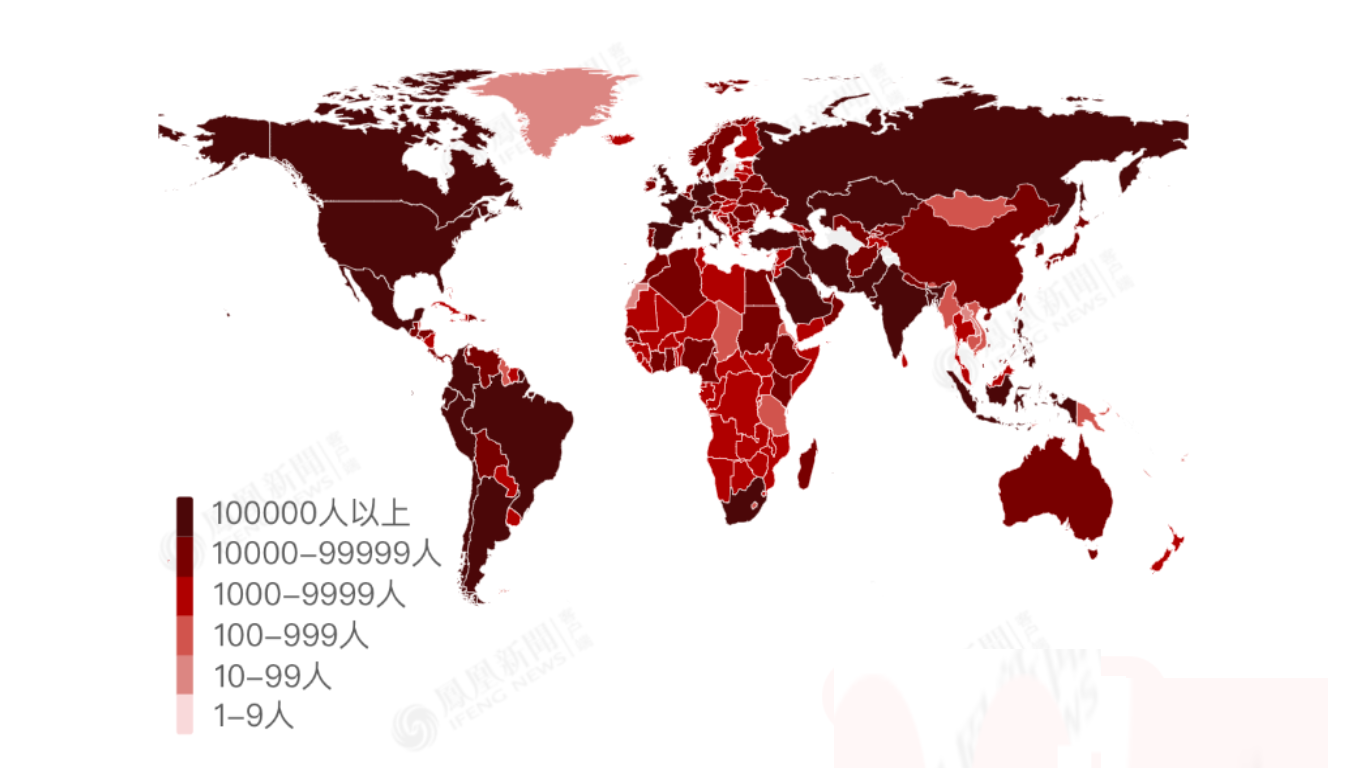
\includegraphics[width=0.6\textwidth]{globalmap.png}
	\caption{全球确诊地图}
	\label{globalmap}
\end{figure} 


\subsection{待解决的问题}
\textbf{问题一:}通过建立的模型预测至少两个不同国家或者地区的确诊病例
和死亡病例的变化,分析各个国家或地区卫生部门采取的举措对降低该国家或地区疫情流行程度的影响并做对此做出评论.

\textbf{问题二:}大流行对国民经济发展产生了巨大的影响,收集某一方面经济发展的数据,建立相应的数学模型以预测未来该方面经济发展的趋势.

\textbf{问题三:}基于一二问的模型和预测结果,向相关国家或者地区的卫生部门写一封信,给出对该国或地区的卫生预防建议.


\section{模型假设}
\begin{enumerate}
	\item 不考虑疫情期间国家或地区人口因迁入或迁出,自然出生或死亡的等因素的影响.
	\item 治愈后的患者由于抗体或者防护措施增强等因素,不会再被感染
     \item 隔离后的患者或者易感染者不会传播或感染病毒.

\end{enumerate}


\section{符号说明}
\begin{center}
	\begin{tabular}{cc}
		\toprule[1.5pt]
		符号 & 含义\\
		\midrule[1pt]
        $N$ &国家或地区的总人口\\
		$S$ & 易感染人群人数\\
		$E$ & 潜伏期易感染者\\
		$I$ &已发病但未隔离患者\\
		$Q$ &已发病且已隔离但未被治疗患者\\
		$J$ & 已发病已隔离且正被治疗者\\
		$R$ & 治愈者\\
		$k$ & 潜伏期患者与已发病患者传染强度的比率\\
           $\beta$ & 病毒传播速率\\
		$\varepsilon$ &潜伏期感染者转入未隔离感染者的比例\\
           $\lambda$ &潜伏期感染者转入已隔离感染者的比例\\
           $\theta$  &未隔离感人者转入正在治疗的人群的比例\\
           $\sigma$  &已隔离感染者转入正在治疗的人群的比例\\
           $\gamma$ &正在治疗的已感染者治愈的比例\\
           $\delta$  &未隔离的已感染者的死亡率\\
           $\eta $   &接受治疗的病人的死亡率\\
           $ h $   &自我隔离的易感染者的比例\\
		\bottomrule[1.5pt]
		注:表中未说明的符号以首次出现处为准
	\end{tabular}
\end{center}




\section{问题一模型的建立与求解}
\subsection{问题分析}
问题一要求我们对不同国家或者地区的确诊病例和死亡病例的变化进行预测,我们会对病毒的传播原理做出机理分析,将本地区的人口按照是否感染病毒,是否接受隔离,是否接受治疗等方面进行划分,病毒在不同人群中间的传播规律是不同的,我们将建立微分方程模型用以描述病毒在人口间的传播.
我们画出了问题一的思维导图.如图\ref{mindmap1}.
\begin{figure}[!htbp]
	\centering
	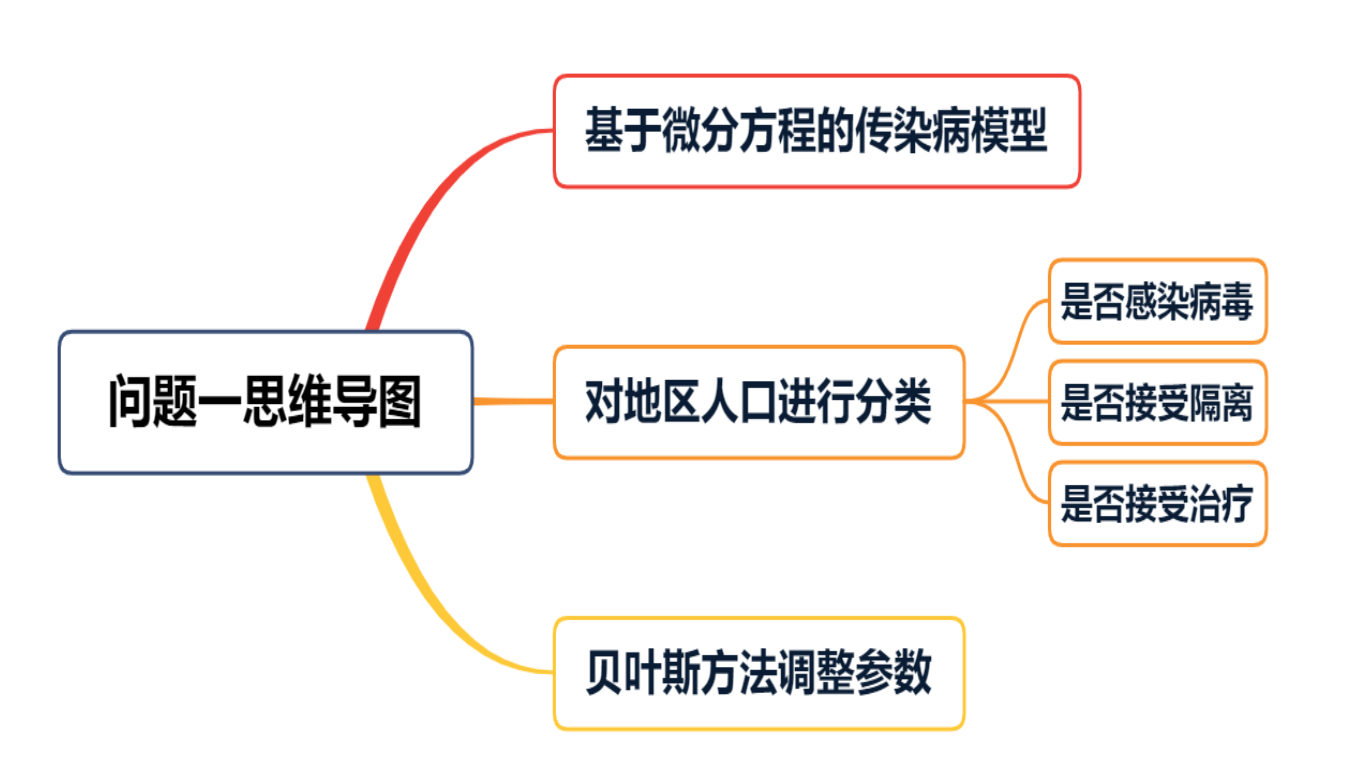
\includegraphics[width=0.6\textwidth]{mindmap1.png}
	\caption{问题一思维导图}
	\label{mindmap1}
\end{figure} 

%插入参考文献\upcite{bib:one}.
\subsection{解决医疗挤兑的传染病动力学微分方程模型}
  为了理清新冠病毒在人群中的传播规律,我们有必要对一些概念作出解释.我们将该地区人口按照感染病毒与否分为易感染者和患者,在本次新冠病毒大流行中,几乎所有年龄阶段的人都有几率感染病毒,老年人感染病毒的几率较大而年轻人较小,但在此我们不对易感染者做出基于年龄,性别等方面的分类.
我们的模型中将人口分为以下几个组,人群之中转变的关系如下图所示.



\textbf{易感染者分组:}
我们假设接受隔离的易感染者与易感染者总数之间存在一个比例关系$h$,易感染者被分为\textbf{未自我隔离}的易感染者$(1-h)S$和\textbf{自我隔离}的易感染者$hS$,$S$为易感染者,即尚未感染的总人口.我们假定只有未隔离的易感者才有感染病毒的风险,这部分易感者可能被潜伏期患者$E$,或已发病且已经隔离但尚未治疗的感染者$Q$感染.$E$人群的传染性比$Q$弱,比例系数$k$处在0-1之间.

\begin{equation}
	\frac{\mathrm{d}S}{\mathrm{d}t}=-(\beta(kE+I)(1-h)S.
\end{equation}
未隔离易感者比例$h$会随着政府的建议或者强制措施而变化.我们假设无隔离政策是所有人气都是未隔离状态,居家令颁布后($t \ge QS$)自我隔离的易感者比例为0.9,即:

\begin{equation}
	h=\begin{cases}
		0,&\text{$t<QS$ }.\\
		0.9,& \text{$t \ge QS$}.
		\end{cases}
\end{equation}

\textbf{易感染者朝感染者的转变:}
据相关研究发现新冠病毒在人体内有一段时间约在的潜伏期,所以易感染者往往不会立即表现出发病状况,而是要在一段时间的潜伏期后才体现出症状,但这时的感染者已经有了轻度传染性.我们用$E$表示已经感染病毒但还在潜伏期的人群,此人群中一部分会被隔离起来,一部分则由于医疗条件的限制或者自身意愿不愿被隔离.
\begin{equation}
 \frac{\mathrm{d}E}{\mathrm{d}t}=\beta(kE+I)(1-h)S-(\varepsilon+\lambda)E.
\end{equation}
其中$I$表示已发病但尚未隔离的感染者,他们具有强传染性,可以将病毒传染给易感染者使其变为潜伏期患者,$Q$表示已发病且已经隔离但尚未治疗的感染者,$\beta$ 被用来表示病毒的传播速率.$\varepsilon$ 和$\lambda$ 分别表示潜伏期患者转入$I$和$Q$的比例关系.
\quad

\textbf{感染者内部:}在感染者内部,经历过一定的潜伏期后,潜伏期患者会出现感染症状,此时他们可能被送入隔离,也可能因为医疗条件或其他原因而无法被隔离.对于没有隔离的已出现症状的感染者,可能会面临死亡风险也可能在后期被送入隔离治疗,隔离治疗的病人组用$J$来表示.
\begin{equation}
\frac{\mathrm{d}I}{\mathrm{d}t}=\varepsilon E-(\theta+\delta)I,
\end{equation}
其中$\theta$表示患者被隔离治疗的比例,而$\delta$表示该组患者的死亡率.

对于被送入隔离的感染者$Q$,它们可能会在一段时间后接受治疗.
\begin{equation}
\frac{\mathrm{d}Q}{\mathrm{d}t}=\lambda E-\sigma Q,
\end{equation}
$\sigma$ 表示该组已感染者转入治疗的比例.

对于被送入隔离治疗环境的患者组$J$,他们可能会在治疗后痊愈并不再感染该病毒,或者面临死亡.
\begin{equation}
\frac{\mathrm{d}J}{\mathrm{d}t}=\theta I+\sigma Q-(\gamma+\eta)J.
\end{equation}
其中$\gamma$表示患者的治愈率,而$\eta$表示该组患者的死亡率.

\quad
\textbf{治愈:}对于患者来说,一旦感染病毒就意味着最终只有两个结果,治愈或者死亡.我们假设治愈着主要来着在医院就诊的患者,参数$\gamma$表示医院的接诊能力或医疗水平,直接影响治愈率:
\begin{equation}
\frac{\mathrm{d}R}{\mathrm{d}t}=\gamma J,
\end{equation}
在我们的\textbf{医疗挤兑模型}中,疾病爆发初期,由于接诊能力,治疗技术和医用物资等因素的限制,医院尚未做好迎接大规模疫情的准备,所以前期一段时间内$0\le t<MUS$保持较低的治愈率$\gamma_0$,出现医疗资源挤兑的情况.然后由于相应的医院扩容,物资补给政策,我们假设医院治疗能力在一段时间$MUS\le t<MUE$内线性增加,直到保持在一个较高的水平$\gamma_1$.
\begin{equation}
	\gamma=\begin{cases}
		\gamma_0,&\text{$0\le t<MUS$ }.\\
		\gamma_0+\frac{(\gamma_1-\gamma_0)(MUE-t)}{(MUE-MUS)},&\text{$MUS\le t<MUE$ }.\\
		\gamma_1,& \text{$MUE \le t$}.
		\end{cases}
\end{equation}

\textbf{死亡:}发病但未隔离的患者$I$和治疗中的患者$J$每天都有一定比率死亡:
\begin{equation}
\frac{\mathrm{d}D}{\mathrm{d}t}=\delta I+\eta J.
\end{equation}
显然上述微分方程组满足如下约束,该地区的总人口(用各个人群之和进行表示)保持不变.
\begin{equation}
N=S+E+I+Q+R+D.
\end{equation}
\begin{equation}
\frac{\mathrm{d}N}{\mathrm{d}t}=0.
\end{equation}

经过前面的推导,我们已经为系统内各人群的数量变化建立\textbf{常微分方程}模型.

\textbf{模型综合}

 \begin{equation}\left\{
	 \begin{array}{l}
	\frac{\mathrm{d}S}{\mathrm{d}t}=-(\beta(kE+I)(1-h)S,\\
	\frac{\mathrm{d}E}{\mathrm{d}t}=\beta(kE+I)(1-h)S-(\varepsilon+\lambda)E,\\
	\frac{\mathrm{d}I}{\mathrm{d}t}=\varepsilon E-(\theta+\delta)I,\\
	\frac{\mathrm{d}Q}{\mathrm{d}t}=\lambda E-\sigma Q,\\
	\frac{\mathrm{d}J}{\mathrm{d}t}=\theta I+\sigma Q-(\gamma+\eta)J,
		\\
	\frac{\mathrm{d}R}{\mathrm{d}t}=\gamma J,\\
	\frac{\mathrm{d}D}{\mathrm{d}t}=\delta I+\eta J.\\
	
	\end{array}\right.
  \end{equation}


\subsection{模型求解}
对于各个地区,微分方程模型的参数各不相同.我们根据实际统计的确诊,死亡,治愈人数,与输出的解比较,定义出损失函数.然后依据损失函数对模型的参数进行调优.
	\subsubsection{数据预处理}
	我们使用附件1,来着约翰·霍普金斯大学系统科学与工程中心(CSSE)的COVID-19数据存储库作为待研究地区确诊,死亡,治愈人数的参考.附件1给出了各地区按天统计的累计确诊,死亡,治愈病例数.我们差分计算出每日新增的病例数,并计算每周7日的滑动平均值.以安徽省数据为例,数据处理的结果见图\ref{fig:Anhui_provinceDF}.
	\begin{equation}
		\Delta D_i = D_{i+1}-D_i,
		\Delta C_i = C_{i+1}-R_i,
		\Delta R_i = R_{i+1}-R_i.
	\end{equation}
	\begin{equation}
		\begin{aligned}
		DMA_i = \frac{\sum_{p=i}^{i+w} D_{p}}{w},\\
		CMA_i = \frac{\sum_{p=i}^{i+w} C_{p}}{w},\\
		RMA_i = \frac{\sum_{p=i}^{i+w} R_{p}}{w}.
		\end{aligned}
	\end{equation}
	\begin{equation}
		\begin{aligned}
		\Delta DMA_i = \frac{\sum_{p=i}^{i+w} \Delta D_{p}}{w},\\
		\Delta CMA_i = \frac{\sum_{p=i}^{i+w} \Delta C_{p}}{w},\\
		\Delta RMA_i = \frac{\sum_{p=i}^{i+w} \Delta R_{p}}{w}.
		\end{aligned}
	\end{equation}
	其中$\Delta D_i,\Delta C_i,\Delta R_i$为第$i$天新增确诊,死亡,治愈的人数,$\Delta DMA_i,\Delta CMA_i,\Delta RMA_i$为$i$到$i+w$天新增确诊,死亡,治愈的人数均值,$w$为滑动平均的窗口大小.
	\begin{figure}[!h]
		\centering
		\includegraphics[width=0.99\textwidth]{Anhui_provinceDF}
		\caption{安徽省确诊,死亡,治愈病例数据}
		\label{fig:Anhui_provinceDF}
	\end{figure}
	\subsubsection{贝叶斯参数调优}
	我们将微分方程所有可调节的参数设为$\mathbf{p}$,对于每一个确定的$\mathbf{p}$,我们都能求出微分方程的数值解,即$\Delta D'_i,\Delta C'_i,\Delta R'_i$.这三个数列和真实数据$\Delta D_i,\Delta C_i,\Delta R_i$符合的越好,说明模型的预测能力越强.为了对$\mathbf{p}$进行调优,我们需要定义损失函数为模型预测的每日新增病例与真实数据的绝对值误差:
	\begin{equation}
		L(\mathbf{p})=\frac{1}{n}(\sum_{i} |\Delta D'_i-\Delta D_i|+\sum_{i} |\Delta D'_i-\Delta D_i|+\sum_{i} |\Delta D'_i-\Delta D_i|).
		\end{equation}
	我们仅能对函数$L(\mathbf{p})$在点$\mathbf{x}$进行抽样求值.每次求值都需要对微分方程模型在进行模拟然后计算损失函数,这涉及较大的计算量.
	这类优化是贝叶斯优化技术最有用的领域.贝叶斯优化用较少的采样数目逼近全局最优值.贝叶斯优化包含了关于$L(\mathbf{p})$的先验信念,并用从$L(\mathbf{p})$中抽取的样本更新先验,从而得到一个更好地接近$L(\mathbf{p})$的后验.用于近似目标函数的模型称为“代理模型”.贝叶斯优化还使用了一个“获取函数”,将采样导向可能优于当前最佳观测的区域.
	
	\textbf{代理模型}(Surrogate model)
	我们使用的代理模型是高斯过程Gaussian Process (GP).高斯过程是一个随机过程,其中任意点$\mathbf{x} \in \mathbb{R}^d$被赋予一个随机值$f(\mathbf{x})$,其中是这些变量的有限数量的联合高斯分布:
	\begin{equation}
		p(\mathbf{f} \lvert \mathbf{X}) = \mathcal{N}(\mathbf{f} \lvert \boldsymbol\mu, \mathbf{K})\label{eq1}.
	\end{equation}
	其中$ \mathbf{f} = (f(\mathbf{x}_1),...,f(\mathbf{x}_N)), \boldsymbol\mu = (m(\mathbf{x}_1),...,m(\mathbf{x}_N)) , K_{ij} = \kappa(\mathbf{x}_i,\mathbf{x}_j)$,$m$是均值函数.高斯过程的函数的分布“平滑度”由K定义.

	一个GP的先验$p(\mathbf{f} \lvert \mathbf{X})$可以在观察到一些数据$y$后转化为GP的后验$p(\mathbf{f} \lvert \mathbf{X},\mathbf{y})$,根据:
	\begin{equation}
			p(\mathbf{f}_* \lvert \mathbf{X}_*,\mathbf{X},\mathbf{y})= \int{p(\mathbf{f}_* \lvert \mathbf{X}_*,\mathbf{f})p(\mathbf{f} \lvert \mathbf{X},\mathbf{y})}\ d\mathbf{f}= \mathcal{N}(\mathbf{f}_* \lvert \boldsymbol{\mu}_*, \boldsymbol{\Sigma}_*).
			\label{eq2}
	\end{equation}
	
	GPs定义了我们对目标函数的先验知识,我们可以使用它们来描述关于目标函数的先验信念,例如“平滑性”.GP后验计算成本低,用于在搜索空间中评估哪些采样点可能产生改进.

	\textbf{获取函数}(Acquisition functions)
	在搜索空间中提出采样点是通过获取函数来实现的.获取函数$u(\mathbf{x} \lvert \mathcal{D}_{1:t})$综合权衡利用(exploitation)和勘探(exploration).利用是指在替代模型预测的目标高的地方进行采样,勘探是指在预测不确定性高的地方进行采样.两者会倾向于提高采集函数值,使得获取函数最大化的采样点为下一步的试验点.
	\begin{equation}
		\mathbf{x}_t = \mathrm{argmax}_{\mathbf{x}} u(\mathbf{x} \lvert \mathcal{D}_{1:t-1}).
	\end{equation}

	\textbf{优化算法}(Optimization algorithm)
	贝叶斯优化算法过程如下.

	For $t = 1,2,...$ 重复执行:

	\begin{itemize}
	\item 通过代理模型(GP)求得获取函数(AF)
	\item  通过获取函(AF)数找到下一个采样点$\mathbf{x}_t = \mathrm{argmax}_{\mathbf{x}} u(\mathbf{x} \lvert \mathcal{D}_{1:t-1})$
	\item 对目标函数进行求值 $y_t = f(\mathbf{x}_t) + \epsilon_t$ .
	\item 将样本$(\mathbf{x}_t,y_t)$加入先验样本 $\mathcal{D}_{1:t} = \{\mathcal{D}_{1:t-1}, (\mathbf{x}_t,y_t)\}$ 
	\item 更新代理模型(GP)
	\end{itemize}

	\textbf{预期提升}(Expected improvement)
	定义为:
	\begin{equation}
		\mathrm{EI}(\mathbf{x}) = \mathbb{E}\max(f(\mathbf{x}) - f(\mathbf{x}^+), 0).
	\end{equation}
	其中 $f(\mathbf{x}^+)$ 是目前最优的目标函数值 $\mathbf{x}^+$ 是最优解 $\mathbf{x}^+ = \mathrm{argmax}_{\mathbf{x}_i \in \mathbf{x}_{1:t}} f(\mathbf{x}_i)$. 

	预期提升可以在GP模型下求得解析解:
	\begin{equation}
		\mathrm{EI}(\mathbf{x}) =
		\begin{cases}
		(\mu(\mathbf{x}) - f(\mathbf{x}^+) - \xi)\Phi(Z) + \sigma(\mathbf{x})\phi(Z), &\text{if}\ \sigma(\mathbf{x}) > 0. \\
		0,& \text{if}\ \sigma(\mathbf{x}) = 0.
		\end{cases}
	\end{equation}
	其中:
	\begin{equation}
		Z =
		\begin{cases}
		\frac{\mu(\mathbf{x}) - f(\mathbf{x}^+) - \xi}{\sigma(\mathbf{x})}, &\text{if}\ \sigma(\mathbf{x}) > 0. \\
		0, & \text{if}\ \sigma(\mathbf{x}) = 0.
		\end{cases}
		\label{eq:Z}
	\end{equation}
	式\ref{eq:Z}中的 $\xi$确定优化期间的探究量,较高的$\xi$值将导致更强的探索.$\xi$ 的推荐值是 $0.01$.

	\begin{figure}[!h]
		\begin{minipage}[t]{0.4\textwidth}
		\centering
		\includegraphics[width=0.99\textwidth]{Anhui_loss_time}
		\caption{安徽省微分方程参数调优损失函数}
		\label{fig:Anhui_loss_time}
		\end{minipage}
		\begin{minipage}[t]{0.6\textwidth}
		\centering
		\includegraphics[width=0.99\textwidth]{Anhui_trials}
		\caption{安徽省微分方程参数调优试验}
		\label{fig:Anhui_trials}
		\end{minipage}
	\end{figure}
	\begin{figure}[!h]
	\end{figure}
  
\subsection{结果分析}
	\subsubsection{最佳参数}
	贝叶斯参数优化器在参数空间中进行1000轮参数搜索试验后,为安徽省和海峡群岛的疫情传播情况找到的最优参数见表\ref{tab:parameters}.其中参数搜索范围参考文献\upcite{bib:two}.
	% Table generated by Excel2LaTeX from sheet 'Sheet1'
	\begin{table}[htbp]
		\centering
		\caption{微分方程模型参数}
		\begin{tabular}{crrl}
		\toprule
				& \multicolumn{1}{c}{\textbf{海峡群岛(英国)}} & \multicolumn{1}{c}{\textbf{安徽省}} & 搜索范围 \\
		\midrule
		\textbf{初始易感人数$S_0$} & 26380.72 & 12338.98 & $10^4 \sim 10^5$ \\
		\textbf{$\beta S_0$} & 0.734773 & 0.456662 & $0.3\sim1.0$ \\
		\textbf{$\delta$} & 0.010046 & 0.010046 & $0.01\sim0.1$ \\
		\textbf{$\epsilon$} & $7.84^{-05}$ & 0.046334 & $0\sim0.3$ \\
		\textbf{$\eta$} & 0.003384 & 0.000546 & $0\sim0.01$ \\
		\textbf{$\gamma_0$} & 0.016848 & 0.018348 & $0\sim0.02$ \\
		\textbf{$\gamma1$} & 0.166284 & 0.158608 & $0.12\sim0.22$ \\
		\textbf{开始隔离政策天数} & 58    & 12    & $0\sim 150$ \\
		\textbf{$k$} & 0.692089 & 0.696911 & $0.6\sim0.7$ \\
		\textbf{$\lambda$} & 0.17209 & 0.201207 & $0.15\sim0.21$ \\
		\textbf{开始医疗升级天数} & 87    & 34    & $0\sim 150$ \\
		\textbf{结束医疗升级天数} & 84    & 19    & $0\sim 150$ \\
		\textbf{$\sigma$} & 0.077206 & 0.293288 & $0\sim0.35$ \\
		\textbf{$\theta$} & 0.122481 & 0.162654 & $0.1\sim0.17$ \\
		\bottomrule
		\end{tabular}%
		\label{tab:parameters}%
	\end{table}%
	\newpage

	\subsubsection{结果展示}
	\begin{figure}[!h]
		\begin{minipage}[t]{0.5\textwidth}
		\centering
		\includegraphics[width=.99\textwidth]{Anhui_compareResult}
		\caption{安徽省真实数据及模型预测}
		\label{fig:Anhui_compareResult}
		\end{minipage}
		\qquad
		\begin{minipage}[t]{0.5\textwidth}
		\centering
		\includegraphics[width=.99\textwidth]{Channel_Islands_compareResult}
		\caption{海峡群岛(英国)真实数据及模型预测}
		\label{fig:Channel_Islands_compareResult}
		\end{minipage}
	\end{figure}
	可以看到安徽省(图\ref{fig:Anhui_compareResult})在19天左右,海峡群岛(图\ref{fig:Channel_Islands_compareResult})在84天左右,新增治愈人数陡增,这符合解决医疗挤兑的传染病动力学模型假设,即:
	疾病爆发初期,治愈率$\gamma_0$较低,出现医疗资源挤兑的情况.然后由于相应的医院扩容,物资补给政策,我们假设医院治疗能力增加,直到保持在一个较高的水平$\gamma_1$.
	
	\subsubsection{灵敏度分析}
	除了医疗资源的变化,政府的隔离政策也对疫情的传播有重大影响,当疫情传播开始之后,何时执行居家令(stay-at-home)和就地避难令(shelter-in-place)对确诊人数,死亡人数也有重大影响.我们对安徽省(图\ref{fig:Anhui_hStart_sensitivity})和海峡群岛(图\ref{fig:Channel_Islands_hStart_sensitivity})关于隔离开始时间进行灵敏度分析,分别在模型搜索到最的近似实际考试时间的基础上,分别提前和延迟5天,然后观察新增确诊人数和死亡人数的曲线.我们发现对于安徽省,每提前执行隔离措施5天,新增确诊和死亡率的峰值都下降到50\%左右;对于海峡群岛,每提前执行隔离措施5天,新增确诊和死亡率的峰值都下降到25\%左右.
	\begin{figure}[!h]
		\begin{minipage}[t]{0.5\textwidth}
		\centering
		\includegraphics[width=.99\textwidth]{Anhui_hStart_sensitivity}
		\caption{安徽省隔离开始时间灵敏度分析}
		\label{fig:Anhui_hStart_sensitivity}
		\end{minipage}
		\qquad
		\begin{minipage}[t]{0.5\textwidth}
		\centering
		\includegraphics[width=.99\textwidth]{Channel_Islands_hStart_sensitivity}
		\caption{海峡群岛(英国)隔离开始时间灵敏度分析}
		\label{fig:Channel_Islands_hStart_sensitivity}
		\end{minipage}
	\end{figure}

	\section{问题二模型的建立与求解}
	\subsection{问题分析}
	新冠病毒大流行对世界经济造成了巨大的影响,人们因隔离而无法工作,国家的援助也不能保证市场按原有计划运行,国家经济会在消费,投资,进出口等方面遭遇大幅衰退.为此,我们选择对反映经济体消费能力的社会消费品零售总额进行分析,通过构建灰色预测模型和时间序列模型预测社会消费品零售总额的正常增长,引入消费者信心这一概念,研究在疫情背景下,消费品零售总额与消费者信心的函数关系,消费者信心用居民消费价格指数的变化来表示.
	问题二的思维导图如图\ref{mindmap2}.
	\begin{figure}[!htbp]
		\centering
		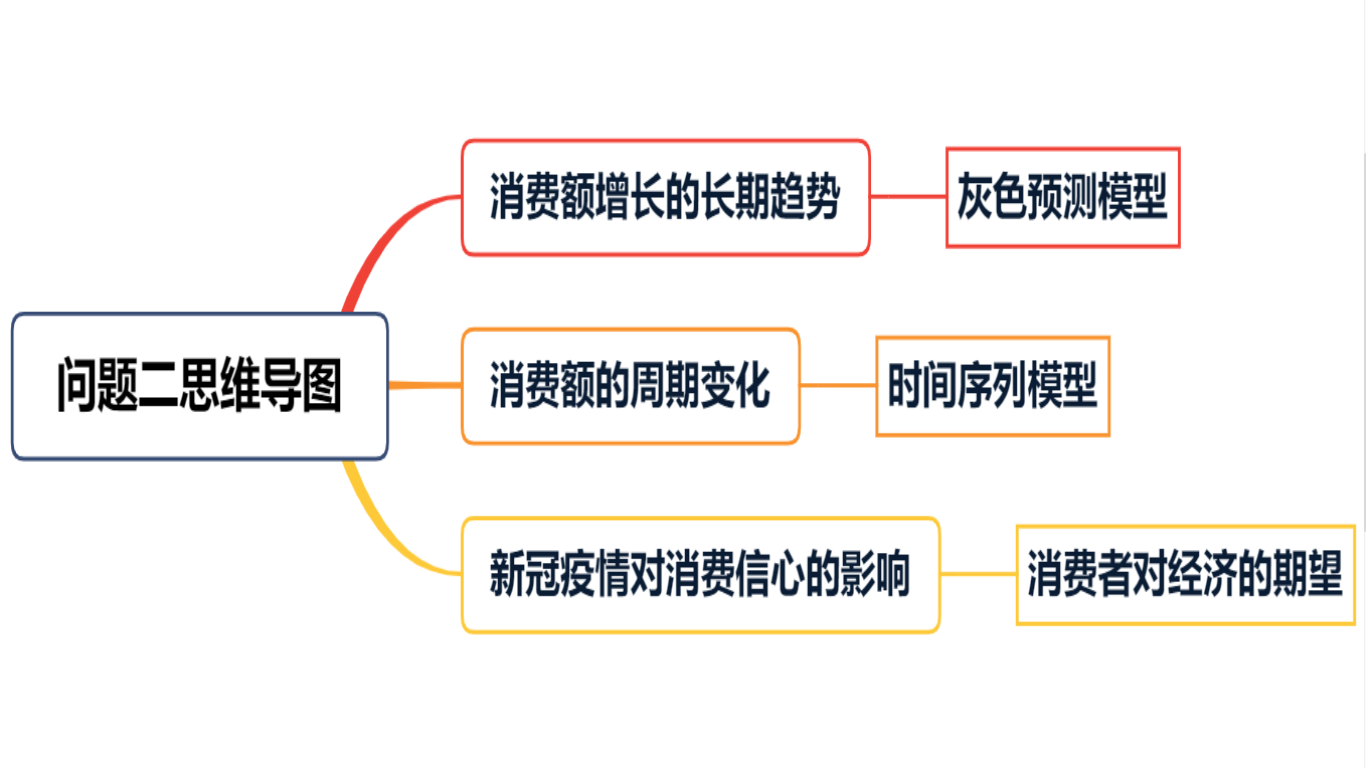
\includegraphics[width=0.6\textwidth]{mindmap2.png}
		\caption{问题二思维导图}
		\label{mindmap2}
	\end{figure} 
	
	
	\subsection{社会消费品零售总额预测模型}
	自2020年1月底新冠病毒大流行爆发以来,由于一系列防控措施所导致的经济封锁,已经在消费,投资与进出口等方方面面影响了社会的经济运转,消费是现代经济社会的支柱,贡献了中国近4成的GDP,消费端因疫情封锁受到的打击会直接影响家庭消费与企业运转,更重要的是会降低民众对经济体的信心,为此我们收集了自2012年以来社会消费品销售总额的数据,对该数据做无疫情影响下的预测分析,然后与受新冠病毒大流行影响的真实数据做对比,以判断消费受到疫情影响的程度.
	
	在中国经济长期增长的背景下,我们认为社会销售品零售额已经由了长期增长的趋势,但作为一般销售品,有其消费增长的周期性规律,这主要体现在不同月份人们消费的需求与喜好的不同.我们认为消费品销售额度$w$由两方面组成,一方面体现在消费品长期增长的趋势$Y$,另一方面体现在消费品受季节影响而导致的波动$T$,我们按照年度及月份从小到大排列,从2015年一月开始编号,$k=1,2,....66$.
	\begin{equation}
	W(k)=Y(k)+T(k).
	\end{equation}
	其中$Y(k)$反映了销售额长期增长的确定性趋势,$T(K)$反映了销售额的季节性随机变化趋势.
	
	
	\subsubsection{销售额长期增长确定性趋势的灰色预测}
	从长远来看,我们的销售额增长趋势整体上是一种稳步上升的趋势,所以本文对于整个销售额的这种确定性增长趋势做灰度预测,本文建立了预测商品销售额长期稳定趋势的一阶线性微分方程GM(1,1).我们用$Y(k)$反映了销售额长期增长的确定性趋势.
	
	\textbf{累加以弱化波动性和随机性:}
	\begin{equation}
	Y^{(1)}=(Y^{(1)}(1),Y^{(1)}(2),...,Y^{(1)}(n)).
	\end{equation}
	其中,n为数据个数.
	\begin{equation}
	Y^{(1)}(t)=\sum_{k=1}^{t}Y^{0}(k),t=1,2,....n.
	\end{equation}
	
	\textbf{生成均值序列:}
	\begin{equation}
	z^{(1)}(k)=\alpha Y^{(1)}(k)+(1-\alpha)Y^{(1)}(k-1)\qquad k=2,3,...n.
	\end{equation}
	
	\textbf{白化微分方程:}
	\begin{equation}
	\frac{\mathrm{d}Y^{(1)}}{\mathrm{d}t}+aY^{(1)}=b.
	\end{equation}
	
	其中$a$为发展系数,$b$为灰色作用量,$a$的有效区间是(-2,2),记$a$,$b$构成的矩阵为:
	\begin{equation}
	\beta={
	\left( \begin{array}{c}
	a\\
	b\\
	.\end{array} 
	\right)}
	\end{equation}
	
	
	\textbf{最小二乘法求解参数:}
	
	\begin{equation}
	\hat \beta=(a,b)^T={(B^{T}B)}^{-1}B^{T}Y_{n}.
	\end{equation}
	
	
	
	\textbf{GM(1,1)离散解:}
	\begin{equation}
	\hat Y^{(1)}(k)=[Y^{(0)}(1)-\frac{b}{a}]e^{-a(k-1)}+\frac{b}{a}, \qquad k=2,3,4...n.
	\end{equation}
	
	\textbf{原始序列预测模型:}
	\begin{equation}
	\hat Y^{(0)}(k)= Y^{(1)}(k)-Y^{(1)}(k-1),\qquad k=2,3,4...n.
	\end{equation}
	\begin{equation}
		\hat Y^{(0)}(k)=[Y^{(0)}(1)-\frac{b}{a}]e^{-a(k-1)}(1-e^a),\qquad k=2,3,4...n.
	\end{equation}
	\subsubsection{销售额的季节性随机变化趋势的时间序列AR模型分析}
	$T(k)$表示数据序列的随机变化趋势因素,通过对2015到2020年的数据进行观察我们可以看出来,销售额增长的过程总是以12个月为周期出现相同的变化趋势,于是我们将$Z(k)=X(k)-Y(k)$的误差变化作为我们销售额的季节变化波动影响.
	
	\textbf{提取周期项}
	\begin{equation}
	L(k)=\begin{cases} 
		0,&k<13. \\
		Z(k)-Z(k-12),&13<k<60.
		\end{cases}
	\end{equation}
	
	\textbf{单位根检验}
	
	我们在使用时间序列之前需要对时间序列的平稳性进行检验,这里采用的ADF检验方法,能够有效判断该序列是否平稳.
	\begin{equation}
		\Delta Z_t=\sigma Z_t-1+\sum_{i=1}^{12}\beta_{i}\Delta Z_{t-i}+\epsilon_t.
	\end{equation}
	零假设 H0:σ=0,原序列存在单位根,为非平稳序列.\\
	备选假设 H1:σ<0,原序列不存在单位根,为平稳序列.
	
	\textbf{样本自相关系数}
	
	样本自相关系数的确定首要条件是该序列为平稳性序列,然后利用协方差的相关性的计算公式,并根据数据代入进行运算.$\hat Z_t$表示的是s周期内的序列$Z_{t-s}$到$Z_t$的均值
	\begin{equation}
	\hat \rho=\frac{cov(Z_t,Z_{t-12})}{\sqrt{Var(Z_t)}\sqrt{Var(Z_t-12)}}=\frac{\sum_{t=s+1}^{T}(Z_t-\overline Z)(Z_{t-s}-\overline Z)}{\sum_{t=1}^{T}(Z_t-\overline Z)^2.}
	\end{equation}
	
	\textbf{样本偏相关系数}
	
	样本偏自相关系数的确定首要条件也是该序列为平稳性序列,然后利用协方差的相关性的计算公式根据数据代入进行运算.最后得到一个关于$\hat{\phi}$的序列.
	\begin{equation}
	P_k=\frac{cov[(Z_t,\hat Z_t),(Z_{t+k}-\hat{Z}_{t+k})]}{\sqrt{Var(Z_t-\hat Z_t)}\sqrt{Var(Z_{t+k},\hat{Z}_{t+k})}},
	\end{equation}
	
	\begin{equation}
	\hat{\phi}_{k+1,k+1}=\frac{\hat{\rho}_{k+1}-\sum_{j=1}^k \hat{\phi}_{kj}\hat{\rho}_{k+1-j}}{1-\sum_{j=1}^k\hat{\phi}_{kj}\hat{\rho}_{k+1-j}}.
	\end{equation}
	
	\textbf{随机波动趋势预测AR序列模型}
	
	根据自相关系数和偏自相关系数的图像,我们可以看到该模型的ACF自相关系数是拖尾形状,而偏自相关系数是截尾情况,从而确定该模型的阶数$\rho=2$
	从而得出该模型的一种表达式情况.其中$\epsilon \sim N(0,\sigma^2)$
	\begin{equation}
	Z_t=\sum_{i=1}^\rho \alpha_i Z_{t-i}+\epsilon.
	\end{equation}
	\subsubsection{消费者缩减支出幅度的分析}
	新冠疫情造成社会经济形势在各方面的恶化,极大打击了消费者的信心,消费者对经济形势保持悲观的情况下,会减少支出以为将来可能的花销做准备.要分析新冠疫情对经济消费端的打击,我们就必须对消费者信心做出预测.
	
	在一个长期增长且稳定的经济体中,消费者价格指数常常保持稳定,因为市场对经济增长有统一却明确的信心,在遭到新冠疫情袭击后,消费者为了抢购物资而推高的消费价格指数,事实上导致了消费品消费额的总体下降,因为售出货品的数量减少的速率大于价格提高的速率.需要指出的是,一次经济危机常导致消费者价格指数先高于基准预期,后低于基准预期,最后走向稳定.
	\begin{figure}[!htbp]
		\centering
		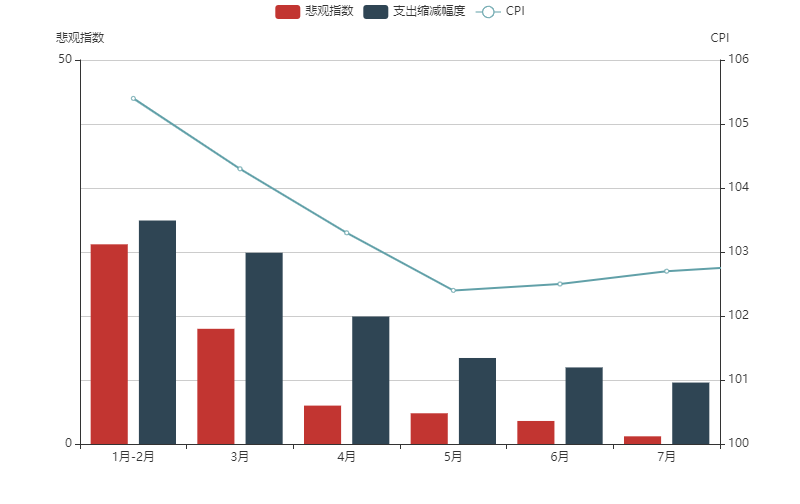
\includegraphics[width=0.6\textwidth]{beiguan.png}
		\caption{2020年以来悲观指数,缩减支出幅度和CPI变化情况}
	\end{figure}
	消费者对经济恶化预期到达某一阈值$F$后,才会做出减少消费的决定,且由于必需品支出无法压缩,消费者压缩支出的幅度$P$不会超出必需品占消费的百分比,此时消费者悲观程度以达到峰值.消费者对于压缩支出的欲望是边际递减的:
	\begin{equation}
	P=\begin{cases}
	0, & D \leq F.\\
	k_{1}lnD+b_{1}, & F<D<=D_{max}.
	\end{cases}
	\end{equation}
	
	$D$表示消费者对经济预期的悲观程度,是消费者信心的反映.$D_{max}$表示悲观程度的峰值,$k_{1}$,$b_{1}$是常数系数,在经济危机期间,消费者信心是趋于悲观的,并以当期$CPI$值$C_{i}$与$CPI$基准值$C_{ave}$之差的绝对值表示.
	\begin{equation}
	D_{i}=|C_{i}-C_{ave}|.
	\end{equation}
	
	\subsection{模型求解}
	\subsubsection{确定性销售额增长GM(1,1)求解}
	\textbf{step1}我们将2015-2019年的每月份销售额原始数据矩阵记为$A_{5\times12}$,代表这5年的60个数据.从而计算出他们的平均值
	$Y_i^{(0)}=\frac{1}{12}\sum_{j=1}^{12} a_ij,i=1,2..5.$
	在生成均值序列是,我们的参数$\alpha=0.5$
	
	\textbf{step2}在白化微分方程的迭代下,通过最小二乘法的计算求得$\beta=(a,b)^T$,从而求得发展系数$a=-0.0061095,b=24666.8866$
	从而得到该灰色模型的离散解
	\begin{equation}
	\hat Y^{(1)}(k)=4059060.67e^{0.0061095(k-1)}-4037464.05,\qquad k=2,3,4...n.
	\end{equation}
	然后取k=6,从而估算出在灰度预测下的确定性增长幅度的均值预测$\hat{Y}^{(0)}(6)=37586.9425$
	
	\textbf{step3}在求出原始数列的预测模型后,我们利用前5年的各月销售额数据,计算出每月销售额所占的比例$\left( r_1,r_2,...r_{12}\right) $
	\begin{equation}
	r_j=\frac{\sum_{i=1}^5a_{ij}}{\sum_{i=1}^{5}\sum_{j=1}^12a_{ij}}.
	\end{equation}
	从而得到各月销售额确定性的分配比例 
	$r=(0.0807, 	0.0814 ,	0.0818, 	0.0821, 	0.0825, 	0.0830, 	$ \\ $	0.0834, 0.0839 ,	0.0843, 	0.0850, 	0.0856, 	0.0864 ) $
	最终得到我们的确定性增长部分的增长数据Y(k)
	\begin{table}[!htbp]
		\caption{销售额确定性增长部分的销售额灰度预测结果} \centering
		\begin{tabular}{cccccc}
			\toprule[1.5pt]
			月份 & 销售额预测 & 月份 & 销售额预测& 月份 & 销售额预测\\
			\midrule[1pt]
			1 & 36390.14264&	5 &37233.4705 &9&	38027.79963	\\
			2 &36696.2505&	6 &37431.51006&10&		38332.88239	\\
			3 &36875.2686& 7 &37622.22469	&11&		38629.19532	\\
			4 &37029.70192&	8&	37822.66108 &12&		38952.20202\\	
			\bottomrule[1.5pt]
		\end{tabular}
	\end{table}
	
	
	
	\subsubsection{周期性随机波动的时间序列求解}
	\textbf{step1平稳性检验:}将灰度预测的模型对其原始数据进行残差波动计算,得到T(t)通过对原始序列的趋势观察和ADF检验我们得出了,利用matlab的adftest函数可以得出\textbf{该模型adf=1,属于平稳性时间序列.}
	
	%\begin{figure}[!htbp]
	%	\centering
	%	\includegraphics[width=0.5\textwidth]{}
	%	\caption{}
	%	\includegraphics[width=0.5\textwidth]{}
	%	\caption{}
	%	
	%\end{figure}
	
	\textbf{step2定阶:}在该模型为平稳性序列的基础上,使用autocorr和parcorr函数,进一步得出了该模型的自相关系数和偏自相关系数的图像,根据图像信息可知该模型的自相关系数呈拖尾状,而偏自相关系数呈截尾状,则\textbf{该模型确定为时间序列的AR模型,且他的阶数$\rho=2$}
	
	\begin{figure}[!h]
		\centering
		\begin{minipage}[c]{0.48\textwidth}
			\centering
			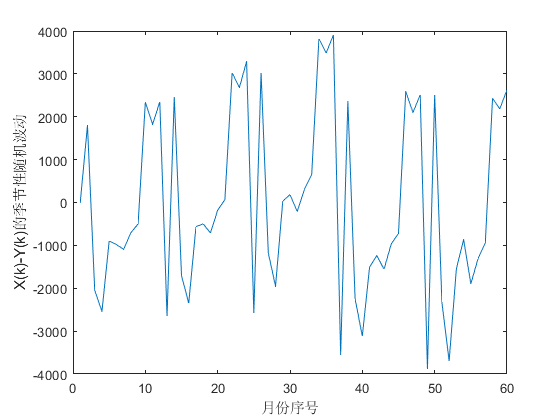
\includegraphics[width=0.99\textwidth]{timeorigin.png}
			\caption{2015-2019年的随机波动}
		\end{minipage}
		\begin{minipage}[c]{0.48\textwidth}
			\centering
			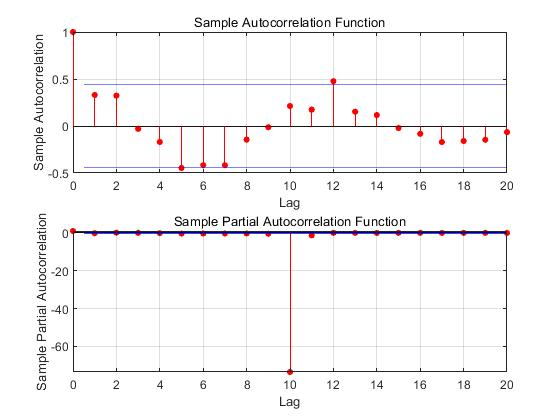
\includegraphics[width=0.99\textwidth]{rhocomfirm.jpg}
			\caption{自相关系数和偏自相关系数图像}
		\end{minipage}
		%	\caption{时间序列模型}
	\end{figure}
	\textbf{step3参数求解:}在确定好我们的时间序列模型为AR模型且$\rho=2$后,我们可以对该时间序列进行拟合和求解,从而计算得出$\alpha_1=-0.6069 \alpha_2=-0.38018 $从而得到未来个月内的波动情况.
	\begin{figure}[!htbp]
		\centering
		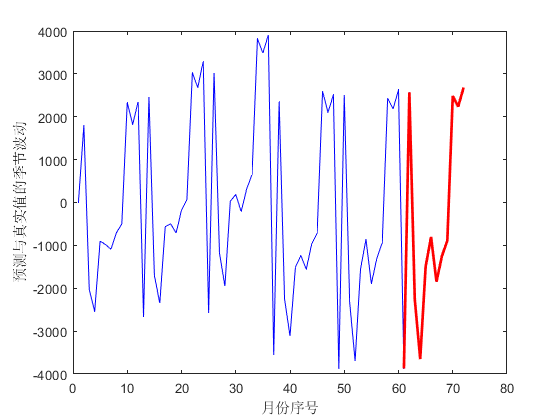
\includegraphics[width=0.6\textwidth]{time.png}
		\caption{2020年的波动预测}
	\end{figure}
	
	最终得到我们的周期性随机波动的增长数据T(k)
	\begin{table}[!htbp]
		\caption{销售额确定性增长部分的销售额灰度预测结果} \centering
		\begin{tabular}{cccccc}
			\toprule[1.5pt]
			月份 & 销售额波动预测 & 月份 & 销售额波动预测 & 月份 & 销售额波动预测\\
			\midrule[1pt]
			1&-3871.939676&	5&-1497.852934&9&-887.4429241\\
			2&2567.104346&	6&-802.965961&10&2484.516924 \\
			3&-2259.204392&	7&-1845.352286&11&2237.164318\\
			4&-3652.111398&	8&-1252.244212&12&2681.111115\\
			\bottomrule[1.5pt]
		\end{tabular}
	\end{table}
	
	
	\subsubsection{悲观缩减支出与悲观程度的拟合}
	我们以2015年至2019年CPI的基准值102.8为判断经济复苏的依据,数据来源于国家统计局,东方财富网等相关网站,在大流行期间,根据时间序列模型拟合的消费者预期消费增长率与现实增长率的差值$P_{i}$,以及每个月消费者的悲观程度$D_{i}$,我们依据2020年1月到5月的数据进行拟合,发现$P$与$D$满足以下函数关系:
	\begin{equation}
	P=9.0627ln(D)+21.102.
	\end{equation}
	用2020年6月份数据进行检验,2020年6月消费者对支出缩减的预估是9.97\%,根据时间序列模型求出的该月8.1\%的增长,我们得到2020年6月预计增长率为-1.87\%,与实际增长率-1.8\%十分接近,证明我们的预测效果较好,根据2020年7月消费者悲观程度计算,我们得到消费者的实际支出会增加0.4\%,这说明经济已经步入复苏阶段,2020年7月社会消费品零售总额预估为33205亿元.
	
	\subsection{结果分析}
	\subsubsection{结果展示}
	经过上述3个方面得模型预测影响,最终我们得到了我国在当前疫情影响下得结果,经过对疫情和时间序列得模拟我们可以得出,当前疫情形势下,我国销售额变化呈现出了先迅速降低,然后随着疫情的慢慢褪去以及消费者信心指数的提升,我们可以看出来当前疫情形势下在7月时达到了同年的相同增长情况,借此我们可以认为从2020年7月开始,我国的销售额恢复达到了2019年的水平,且各项指标都将回复成时间序列下的常规状态,借此我们可以利用波动规律对之后的2019年数据进行有效预测,得到下半年各月之间的销售额分别为33525.9,33205,34028,34626.6,38225.68,38908.4亿元.
	\begin{figure}[!htbp]
		\centering
		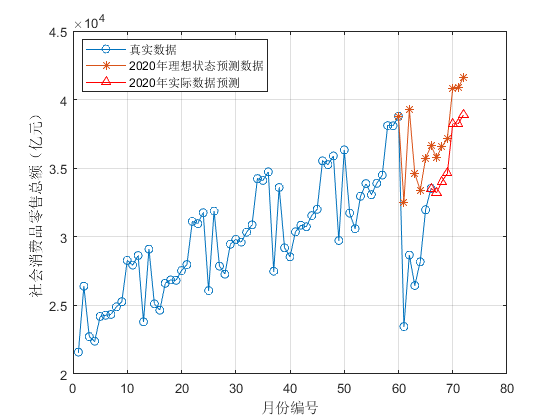
\includegraphics[width=0.6\textwidth]{pred4.png}
		\caption{2020年的销售额实际预测与理想预测的对比}
	\end{figure}
	
	\begin{table}[!htbp]
		\caption{2020年的下半年销售额预测情况} \centering
		\begin{tabular}{cccccc}
			\toprule[1.5pt]
			月份 & 预测销售额  &月份 & 预测销售额\\
			\midrule[1pt]
			7&33525.9&	10&34626.6\\
			8&33205&	11&38225.68\\
			9&34028&	12&	38908.4\\
			\bottomrule[1.5pt]
		\end{tabular}
	\end{table}
						
	\subsubsection{灰度预测模型检验}
	我们的灰度预测拟合度具有准指数的性质,光滑比小于0.5的数据占比为$98.3051\%$除去前两个时期外,光滑比小于0.5的数据占比为$100\%$,平均相对残差为0.061574,平均级比偏差为0.066514表明其拟合效果很好,因此在确定性趋势下的
	\begin{figure}[!htbp]
		\begin{minipage}[t]{0.5\textwidth}
		\centering
		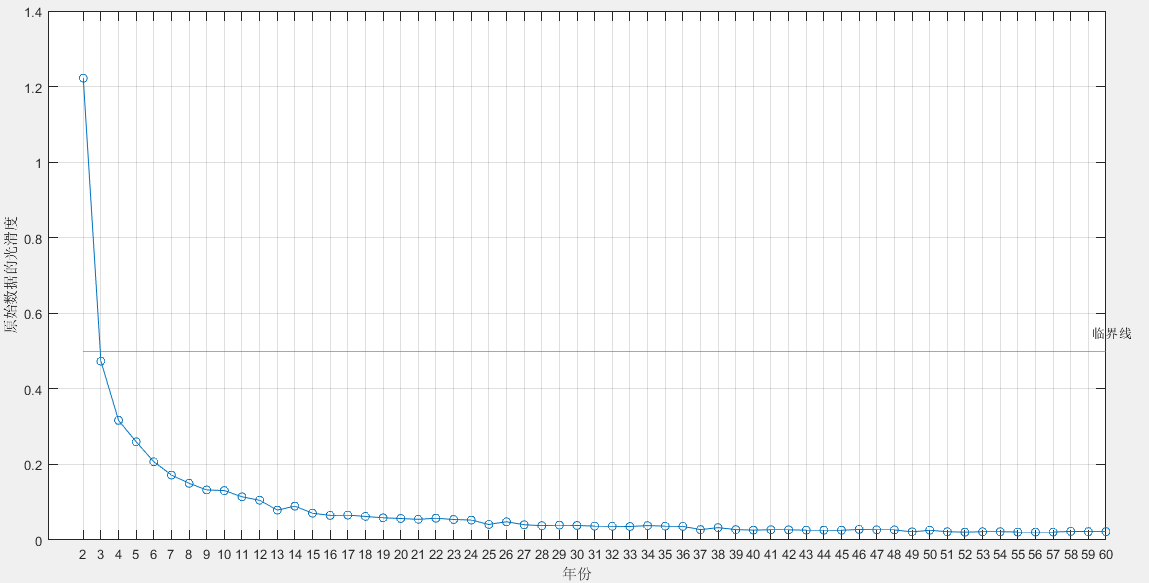
\includegraphics[width=0.99\textwidth]{pinhua.png}
		\caption{灰度预测各个平滑度}
		\end{minipage}
		\qquad
		\begin{minipage}[t]{0.5\textwidth}
		\centering
		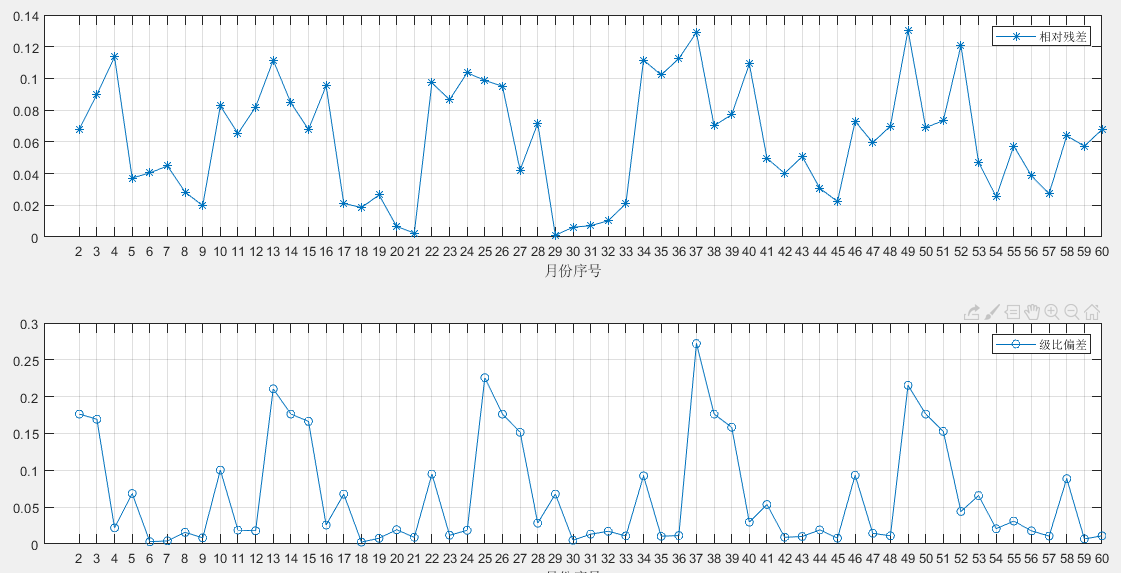
\includegraphics[width=0.99\textwidth]{huidumse.png}
		\caption{灰度预测相对残差和级比残差}
		\end{minipage}
	\end{figure}
	\subsubsection{自回归残差检验}
	自回归标准残差,基本在0的附近,而他的QQ图残差基本完全落在45°线上,表明确实是符合其正态分布的假设.且AR(2)的定阶对应的BIC值是最小的.
	
	\begin{figure}[!htbp]
		\begin{minipage}[t]{0.5\textwidth}
			\centering
			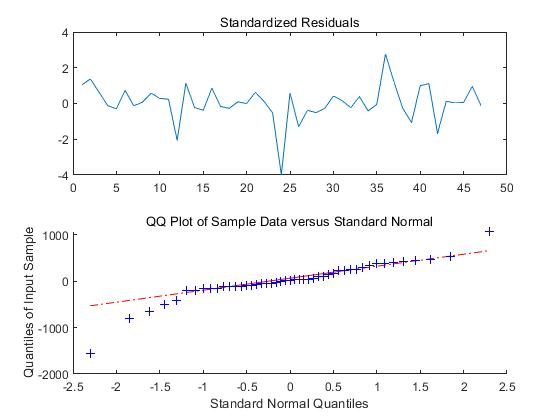
\includegraphics[width=0.99\textwidth]{qq.jpg}
			\caption{标准化残差与QQ图正态检验}
		\end{minipage}
		\qquad
		\begin{minipage}[t]{0.5\textwidth}
			\centering
			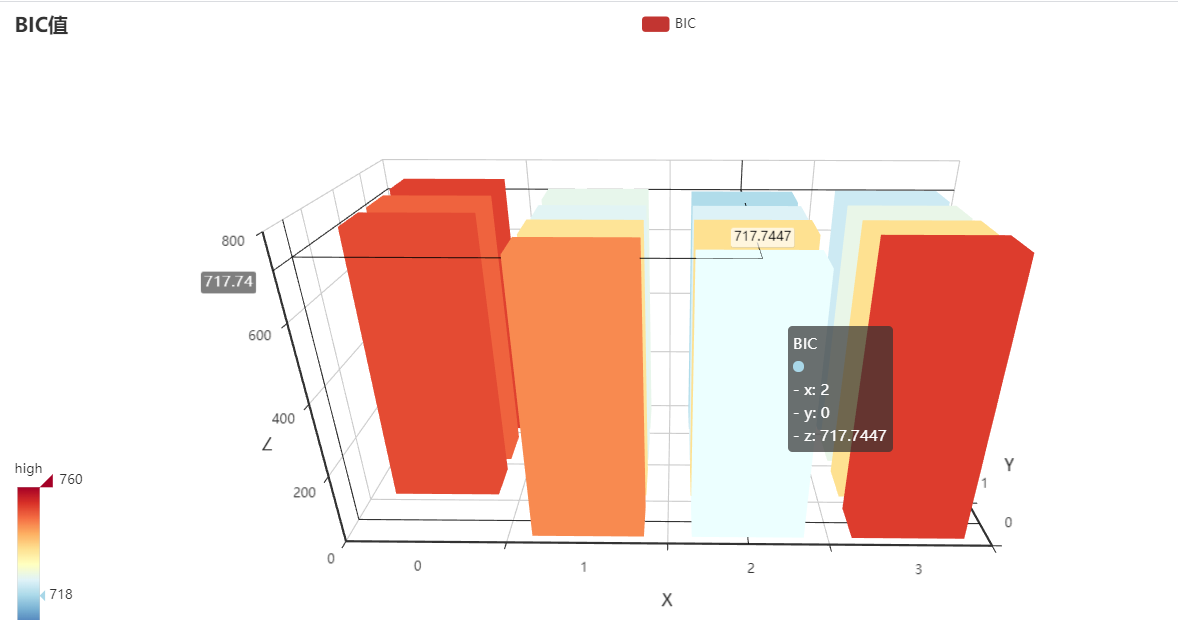
\includegraphics[width=0.99\textwidth]{bci.png}
			\caption{定阶对应的BIC值}
		\end{minipage}
	\end{figure}
	\newpage
	\section{模型评价}
	\subsection{模型的优点}
	1.在建立改进的SEIR模型是,考虑了愿意自我隔离的人的比例随疫情发展情况的变化,通过对病毒传播的机理分析,我们依据隔离与治疗与否,将感染者细分成三类,考虑到了患者送医时间,隔离比例对病毒传播的影响,对传播过程模拟的仿真度高.
	
	2.问题二模型考虑了消费增长的趋势性与周期性因素,研究疫情对经济的短期影响时,引入了消费者悲观程度,并作出了经济学解释,模型与真实经济发展状况契合程度较高.
	
	\subsection{模型的缺点}
	1.由于缺少数据,无法对感染者进行进一步分类,感染者按照病情发展程度,其治愈率,死亡率,传播病毒能力都是不同的,如果有更详细的数据,我们可以将模型进一步完善.
	
	2.由于缺少资料,未就疫情后经济复苏的潜力进行量化.
	
	\subsection{改进与展望}
	已有不少学者应有对传统SEIR模型提出改进,魏等\upcite{bib:two}提出了对已发病感染者按照轻症,中度和重症进行分类,使用马尔科夫链蒙特卡洛算法结合Gibbs抽样的方法得到了更准确的参数,模型拟合效果较理想.在模型建立过程中,没有考虑到人口迁入迁出的影响,晏等\upcite{bib:seven}对新冠肺炎感染人群做了人口学分析,可以参考他们的结论进一步完善模型,.
	
	
	\section{致国家卫生部门的一封信}
	\textbf{尊敬的卫生部门领导:}
	
	您好.
	
	新冠病毒大流行已经造成了全球范围内严重的公共卫生危机,各国已经为战胜危机付出了巨大努力,各国应对新冠病毒的措施包括但不限于发布居家令,建立发热门诊,建设专门应对病毒的临时医院,强制佩戴口罩,研发特效药与疫苗.目前,全球范围内的病毒传播还处于扩散阶段,这主要是因为部分国家防控意识薄弱,医疗水平落后,且国际援助水平有限.为了更快且彻底的摆脱新冠病毒危机,我们对新冠病毒的传播过程进行建模并分析,根据所得结果向贵部门提出相应建议:
	
	1.立刻出来相应法规隔离养老院等老年人集聚地并提供帮助,全球新冠肺炎患者中,60岁及以上年龄患者占一半以上,加强对老年人的保护能够有效切断病毒在人际间的传播.
	
	2.加强医疗卫生投入,对已发病或者潜伏期但已检测为阳性的患者应收尽收,我们发现提高收治效率能够显著降低新增感染人数.
	
	3.尽快发布居家隔离令,强制居民在家隔离,可以有效降低前期感染人数,尽早压平感染曲线.
	
	4.展开大规模的病毒筛查,建立分级诊断机制,将人群中的潜伏期患者找出,避免造成易感人群的规模性的群体感染.只有找出所有潜伏期患者,新冠病毒传播的源头才能被阻隔.
	
	5.传统的防控手段并不能使全部人口免于病毒感染,应加快对该病毒特效药和疫苗的研发,易感染人群越早完成疫苗的接种,病毒就能更早的被全面控制.
	
	
	希望我们做的调查和预测能为您提供一些有效信息,为抗击疫情献上我们的绵薄之力,同时我们衷心祝愿我国能够早日战胜新冠疫情,恢复正常生活,加快全面小康的进程.
	
	
		

\appendix %%附录
\begin{thebibliography}{9}%宽度9
	\bibitem{bib:one}陈柯宇.基于SEIR模型的新型冠状病毒疫情实证分析[J].统计与管理,2020,35(06):31-38.
	\bibitem{bib:two}魏永越, 卢珍珍, 杜志成, 张志杰, 赵杨, 沈思鹏, 王波, 郝元涛, 陈峰. 基于改进的SEIR+CAQ传染病动力学模型进行新型冠状病毒肺炎疫情趋势分析[J]. 中华流行病学杂志, 2020, 41(4): 470-475.
	\bibitem{bib:three}徐致靖. 复杂社会系统中的传染病动力学建模与案例研究[D].中国人民解放军军事医学科学院,2015:34-25.
	\bibitem{bib:four}颉俊慧. 两类传染病动力学建模与分析[D].山西大学,2017:7-11.
	\bibitem{bib:five}Arapović Jurica,Skočibušić Siniša. The first two months of the COVID-19 pandemic in Bosnia and Herzegovina: Single-center experience.[J]. Bosnian journal of basic medical sciences,2020,20(3).
	\bibitem{bib:six}Carlos Victor Chaves de Lima,Estelita Lima Cândido,José Arinelson da Silva,Letícia Viana Albuquerque,Lívia de Menezes Soares,Mayara Maciel do Nascimento,Sara Alves de Oliveira,Modesto Leite Rolim Neto. Effects of quarantine on mental health of populations affected by Covid-19[J]. Journal of Affective Disorders,2020,275.
	\bibitem{bib:seven}晏月平,李忠骥.新冠肺炎感染人群的人口学分析——以我国10省市区为例[J].人口与发展,2020,26(03):73-85.

\end{thebibliography}


\section{代码}
\subsection{python源程序}
\lstinputlisting[language=python]{code/main.py}
\lstinputlisting[language=python]{code/common.py}
\lstinputlisting[language=python]{code/paramater_tuning.py}
\lstinputlisting[language=python]{code/read_data.py}
\lstinputlisting[language=python]{code/sensitivity.py}
\lstinputlisting[language=python]{code/solve_scipy.py}
\subsection{matlab源程序}
\lstinputlisting[language=matlab]{code/main.m}
\lstinputlisting[language=matlab]{code/gray.m}
\lstinputlisting[language=matlab]{code/gm11.m}
\lstinputlisting[language=matlab]{code/metabolismgm11.m}
\lstinputlisting[language=matlab]{code/newgm11.m}
\lstinputlisting[language=matlab]{code/time.m}

\end{document}